\documentclass[12pt, a4paper]{article}
    
\usepackage{homework}
\usepackage{amsmath}				% For Math
\usepackage{fancyhdr}				% For fancy header/footer
\usepackage{graphicx}				% For including figure/image
\usepackage{cancel}					% To use the slash to cancel out stuff in work
\usepackage{multirow}

%%%%%%%%%%%%%%%%%%%%%%
% Set up fancy header/footer
\pagestyle{fancy}
\setlength{\headheight}{42pt}
\fancyhead[LO,L]{Name: Yu Ching Hei\\SID: 1155193237\\email: chyu2@cse.cuhk.edu.hk}
\fancyhead[CO,C]{}
\fancyhead[RO,R]{CENG3420 Computer Organization and Design\\Lab 2.2\\Date: \today}
\fancyfoot[LO,L]{}
\fancyfoot[CO,C]{}
\fancyfoot[RO,R]{Page \thepage}
\renewcommand{\headrulewidth}{0.4pt}
\renewcommand{\footrulewidth}{0.4pt}
%%%%%%%%%%%%%%%%%%%%%%

\begin{document}
\begin{qNoMark}
Implement an RISCV-LC ISA Simulator. 
\end{qNoMark}

\begin{ans}
\\\indent In this lab, we are going to complete some of the instructions in the sim.c file. 
There are few main points to mark and it is going to be stated in this lab report. 
In the following part, I am going to demonstrate how I complete this lab. 

Let's say we have to complete the \texttt{handle\_slli} function: 
Since we know that it is a I-type instructions, we can refer to the sample implementation of the \texttt{handle\_addi} function
\begin{code}
void handle_addi(unsigned int cur_inst) {
    unsigned int rd = MASK11_7(cur_inst), rs1 = MASK19_15(cur_inst);
    int imm12 = sext(MASK31_20(cur_inst), 12);
    NEXT_LATCHES.REGS[rd] = CURRENT_LATCHES.REGS[rs1] + imm12;
}
\end{code}
since the parsing is the same for all integer R-I instructions, but only differs by the logic, I just have to modify line 4
by changing the ``\texttt{+}'' operator to other operators like ``$\ll$'' for \texttt{slli}, ``$\wedge$'' for \texttt{ori} etc. 
Basically most integer R-I instructions like \texttt{slli, xori, srli, ori, andi, lui} can be implemented in the same way except \texttt{srai}. 
\\Since the result of \texttt{srai} instruction is MSB-extended, we have to put the result into the \texttt{sext()} fucntion before storing it into the rd. 
\begin{verbatim}
    NEXT_LATCHES.REGS[rd] = sext(CURRENT_LATCHES.REGS[rs1] >> imm5, 32);
\end{verbatim}


\indent Then we have the integer R-R type instructions. These instructions implement R-Type format. So we are refering to the R-Type instruction example
\begin{code}
void handle_add(unsigned int cur_inst) {
    unsigned int rd = MASK11_7(cur_inst),
                rs1 = MASK19_15(cur_inst),
                rs2 = MASK24_20(cur_inst);
    NEXT_LATCHES.REGS[rd] = CURRENT_LATCHES.REGS[rs1] 
                            + CURRENT_LATCHES.REGS[rs2];
}
\end{code}
To complete the R-Type instructions, it shares the same idea of I type, 
by changing the ``\texttt{+}'' operator in line 6 to other operators like ``$\ll$'' for \texttt{sll}, ``$\wedge$'' for \texttt{or} etc. 
Same for R-R instructions, \texttt{sra} requires special handling as it has MSB-extended return value. 
so the last line becomes
\begin{verbatim}
        NEXT_LATCHES.REGS[rd] = sext(CURRENT_LATCHES.REGS[rs1] 
                            >> CURRENT_LATCHES.REGS[rs2], 32);
\end{verbatim}
For unconditional jump \texttt{JAL}, it uses J-Type format which has the 20-bit jimm20 specially formatted into the form 
of $[20|10:1|11|19:12]$. Therefore, there is no simple masking but we have to mask the current instruction binary stream part by part. 
The construction of jump immediate is done as below: 
\begin{code}
int imm20 = (MASK19_12(cur_inst) << 12);
    imm20 += (MASK20(cur_inst) << 11);
    imm20 += (MASK30_21(cur_inst) << 1);
    imm20 += (MASK31(cur_inst) << 20);
\end{code}
then the PC + 4 of current state will be stored into the rd if provided
and the sign-extended jump immediate is added to the current PC as a offset then stored to 
the PC of next state to let the FSM jump to the desire location in the next state

For unconditional jump \texttt{JALR}, is uses I-Type format so it shares the same parsing format as the I-Type as implemented in the previous part. 
But the main different is we are jumping to an address reletive to an address stored in register. Therefore, instead of adding the jump offest directly to the 
next state PC, the next state PC is set to the address stored in rs1 that is offset by the immediate value. 

For conditional branches, there is a given example of beq, so we can just mimic the parsing logic done in beq and change the branching logic
\begin{code}
void handle_beq(unsigned int cur_inst) {
    unsigned int rs1 = MASK19_15(cur_inst), rs2 = MASK24_20(cur_inst);
    int imm12 = (MASK31(cur_inst) << 12) + \
            (MASK7(cur_inst) << 11) + \
            (MASK30_25(cur_inst) << 5) + \
            (MASK11_8(cur_inst) << 1);
    if (CURRENT_LATCHES.REGS[rs1] == CURRENT_LATCHES.REGS[rs2])
        NEXT_LATCHES.PC = (sext(imm12, 12) + CURRENT_LATCHES.PC);
}
\end{code}
we just have to modify the ``\texttt{+}'' in line 8 to implement different branching logic like ``\texttt{!=}'' for \texttt{bne}, ``\texttt{>=}'' for \texttt{bge} and
``\texttt{<}'' for \texttt{blt}. 

For load instructions, they are in I-Type format so the parsing is the same as implemented in the previous part. 
By following the example of the \texttt{lb}, we can formulate the instructions to read the memory from the address that is offset by the immediate. 
After retrieving the value from the memory, I applied corresponding masking fucntion to the value so that the output will be of the desired length. 

For store instructions, they have similar instruction parsing as the conditional branch instructions, so the main focus will be the storing mechanism. 
This is the implementation of my \texttt{handle\_sw} fucntion. 

\begin{code}
void handle_sw(unsigned int cur_inst) {
    unsigned int rs1 = MASK19_15(cur_inst), rs2 = MASK24_20(cur_inst);
    int imm12 = (MASK11_7(cur_inst));
    imm12 += (MASK31_25(cur_inst) << 5);
    int startAddr = CURRENT_LATCHES.REGS[rs1] + sext(imm12, 12);
    MEMORY[startAddr] = (MASK7_0(CURRENT_LATCHES.REGS[rs2]));
    MEMORY[startAddr + 1] = (MASK15_8(CURRENT_LATCHES.REGS[rs2]));
    MEMORY[startAddr + 2] = (MASK23_16(CURRENT_LATCHES.REGS[rs2]));
    MEMORY[startAddr + 3] = (MASK31_24(CURRENT_LATCHES.REGS[rs2]));
}
\end{code}
In my code, I have separated the data to be stored to the memory into 4 different sections and store 
them into the memory byte by byte separately. For word(32-bit), split into 4 chunks; for half(16-bit), split into 2 chunks. 

\end{ans}
\pagebreak
The following are the screenshots of the corresponding similations. 
\begin{figure}[H]
    \caption{add4.bin}
    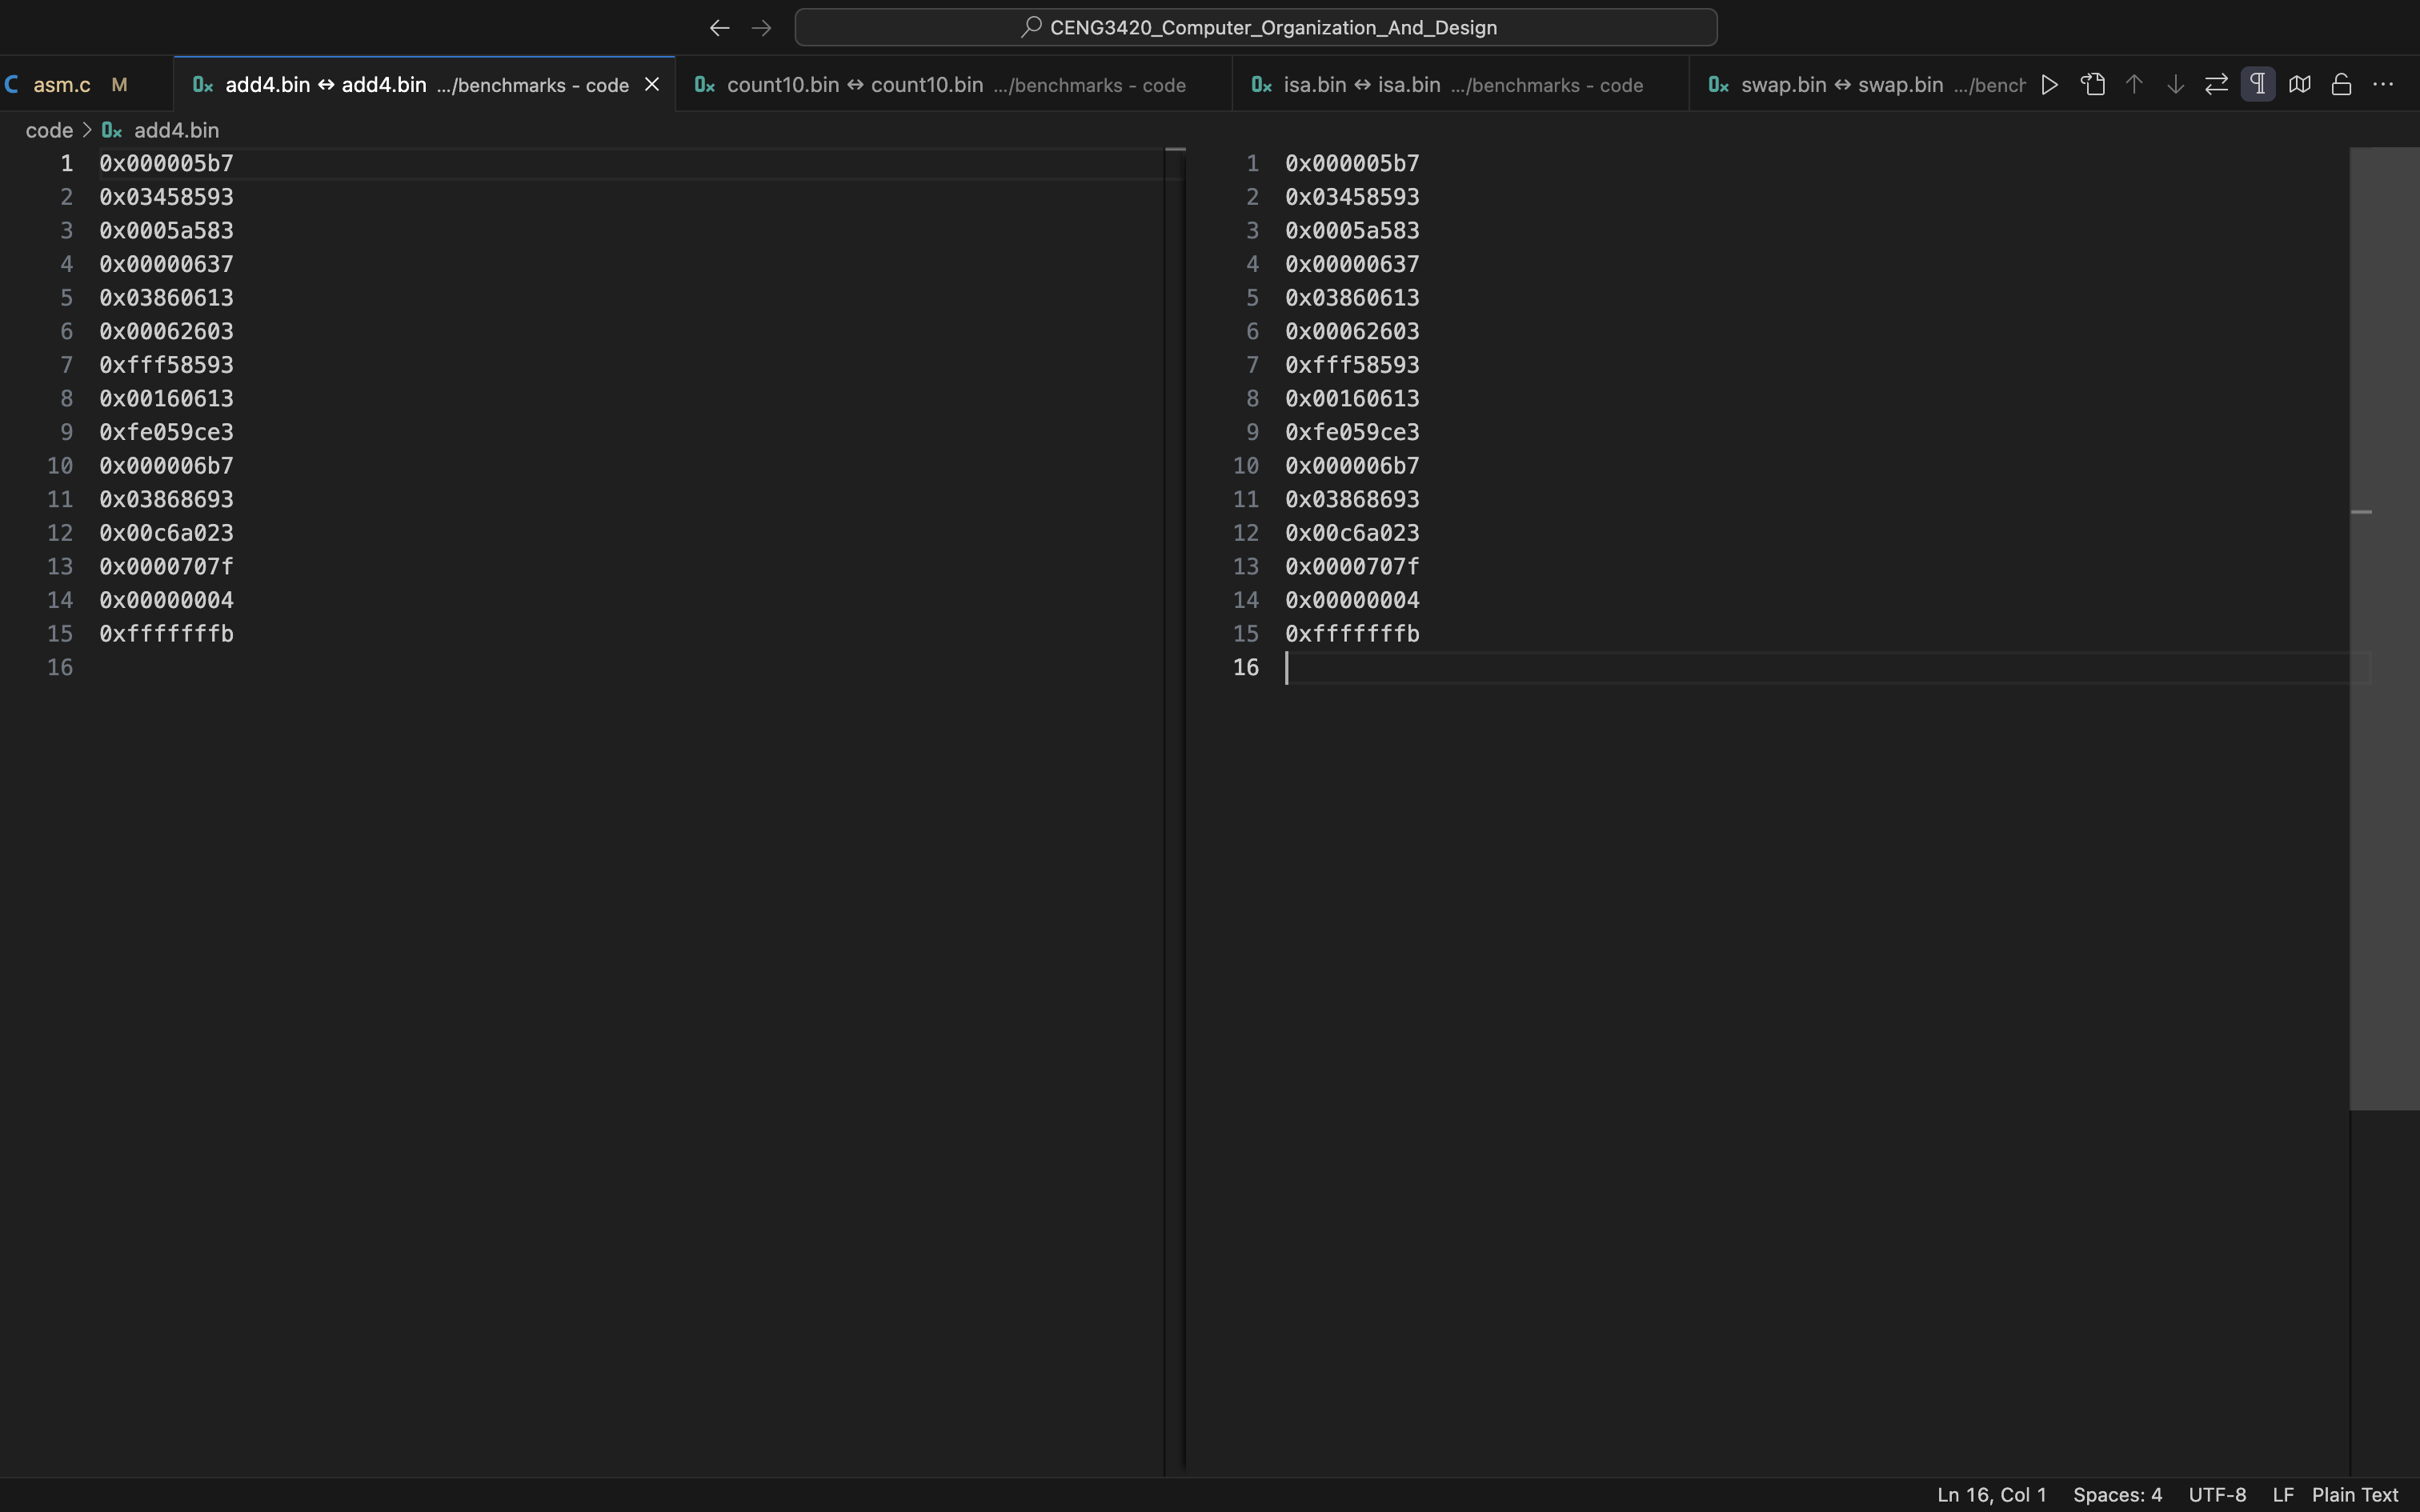
\includegraphics[width=1\linewidth]{../figs/add4.png}
\end{figure}

\begin{figure}[H]
    \caption{count10.bin}
    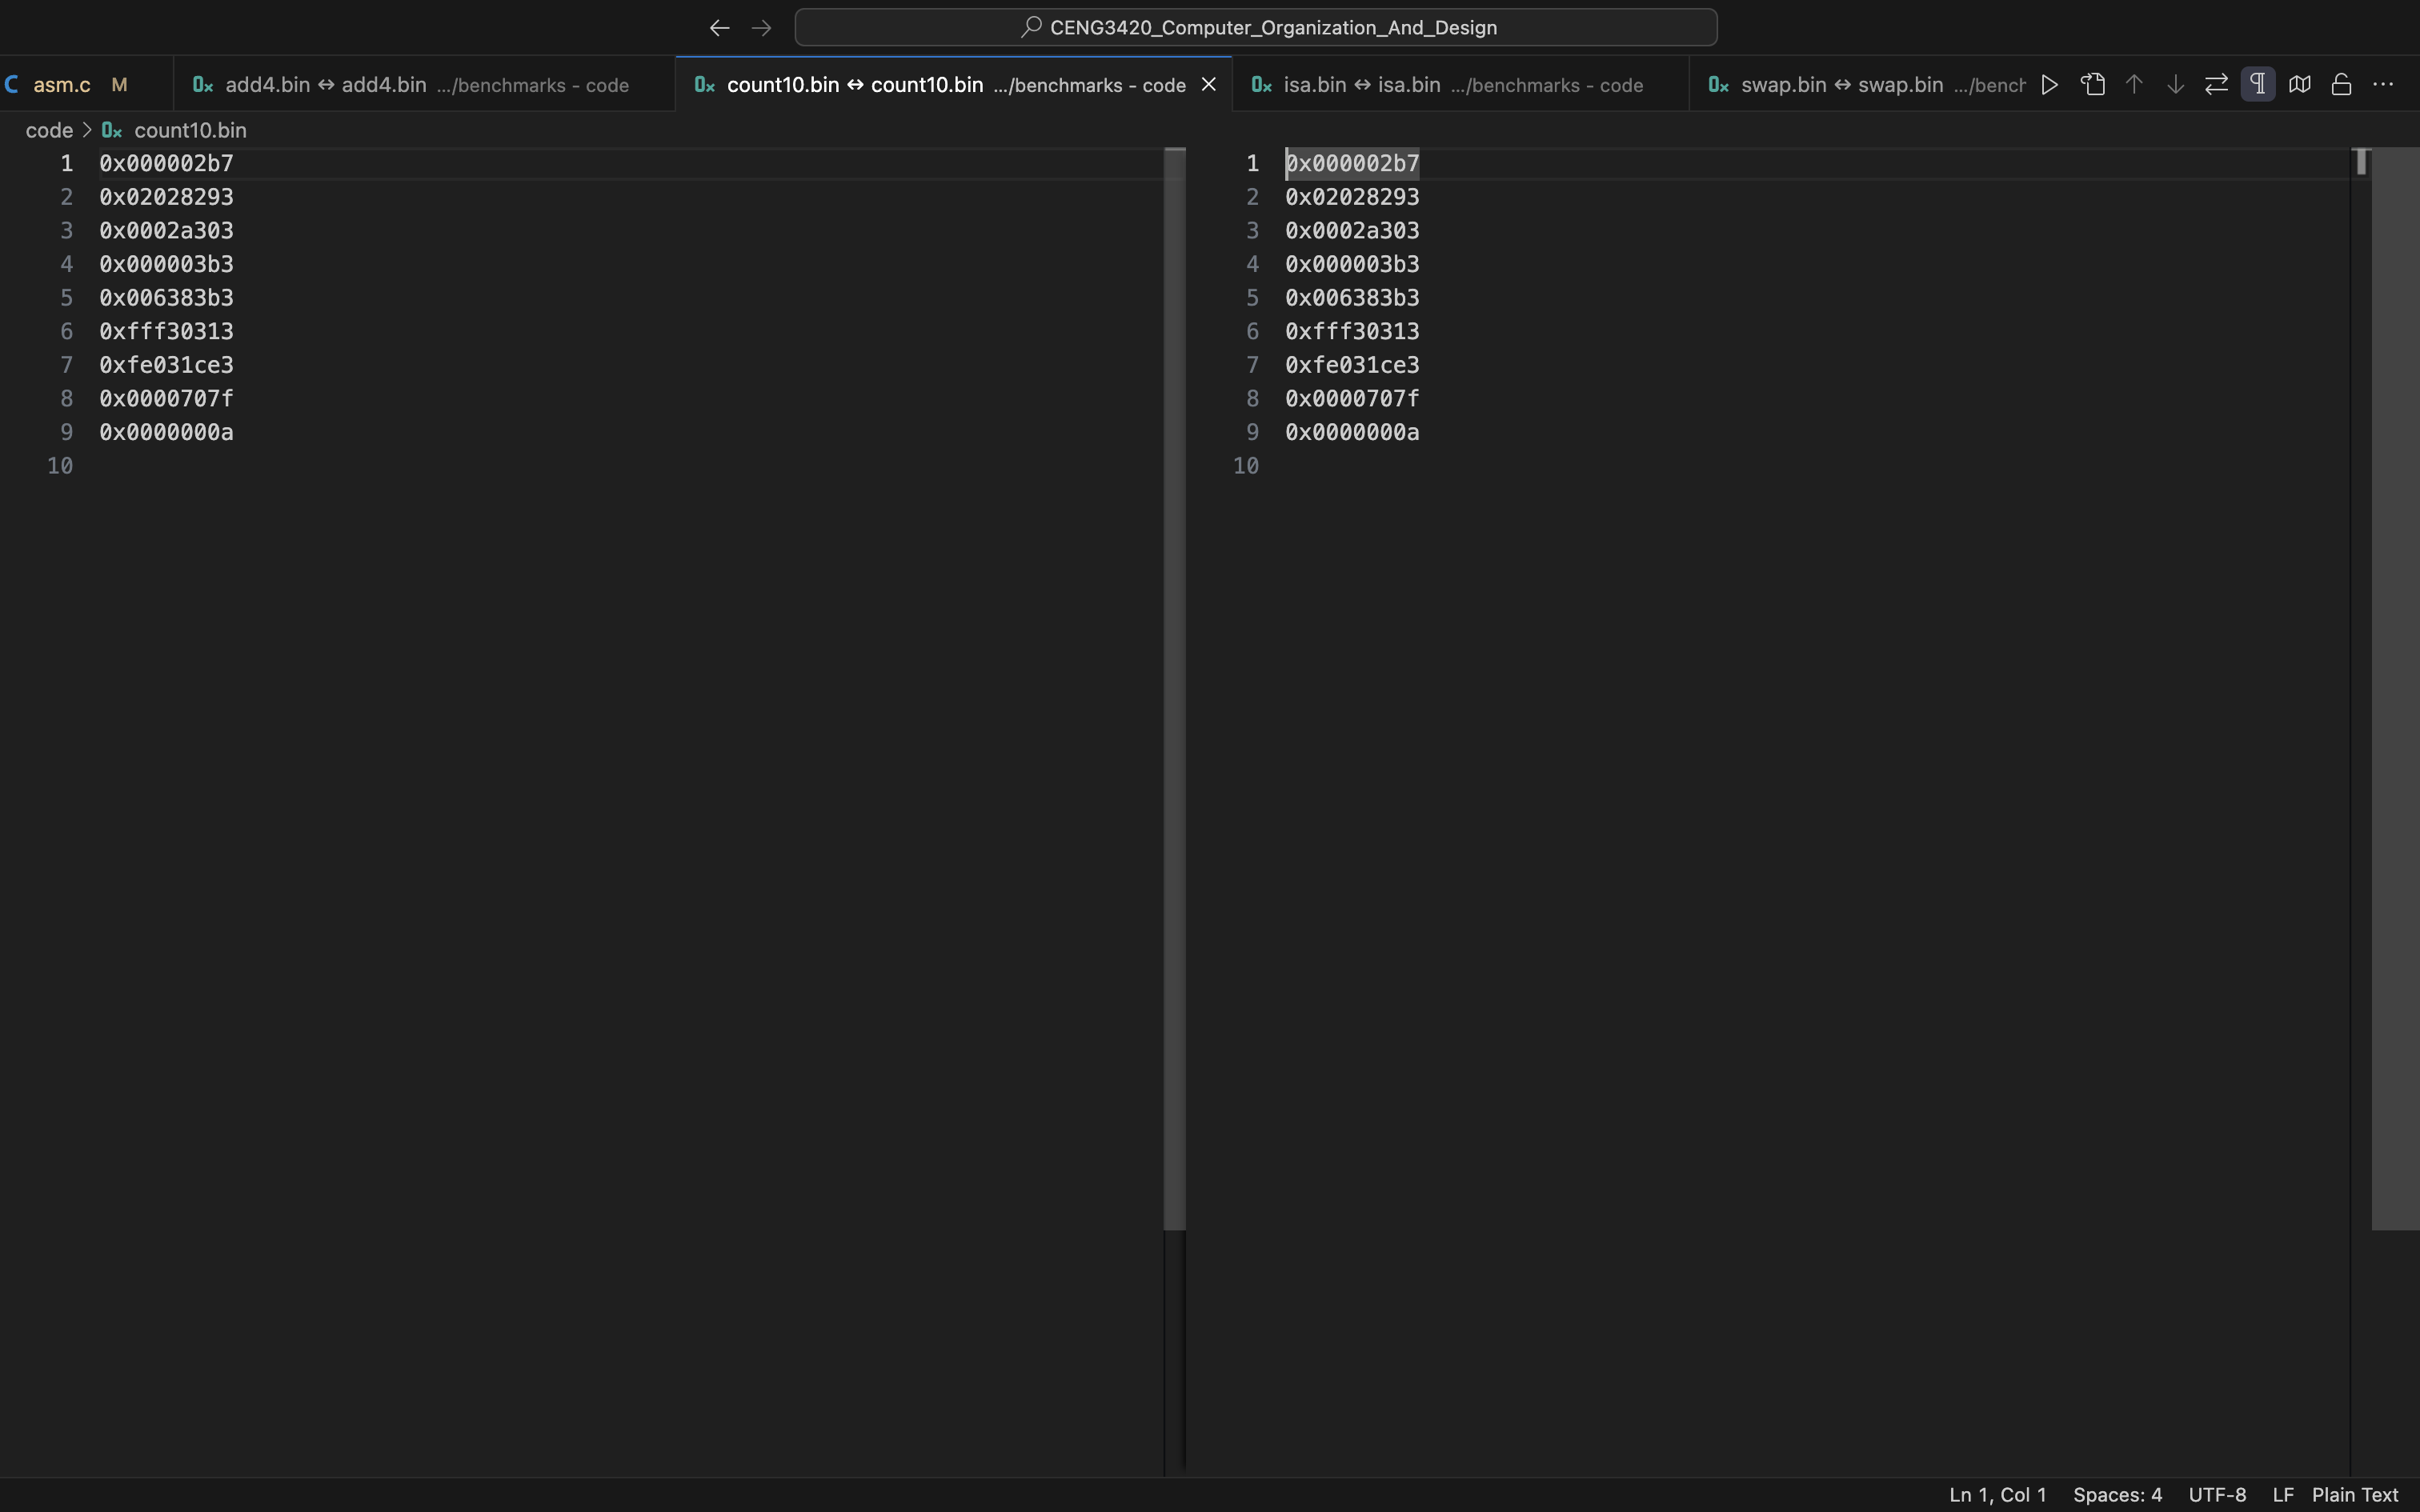
\includegraphics[width=1\linewidth]{../figs/count10.png}
\end{figure}

\begin{figure}[H]
    \caption{isa.bin}
    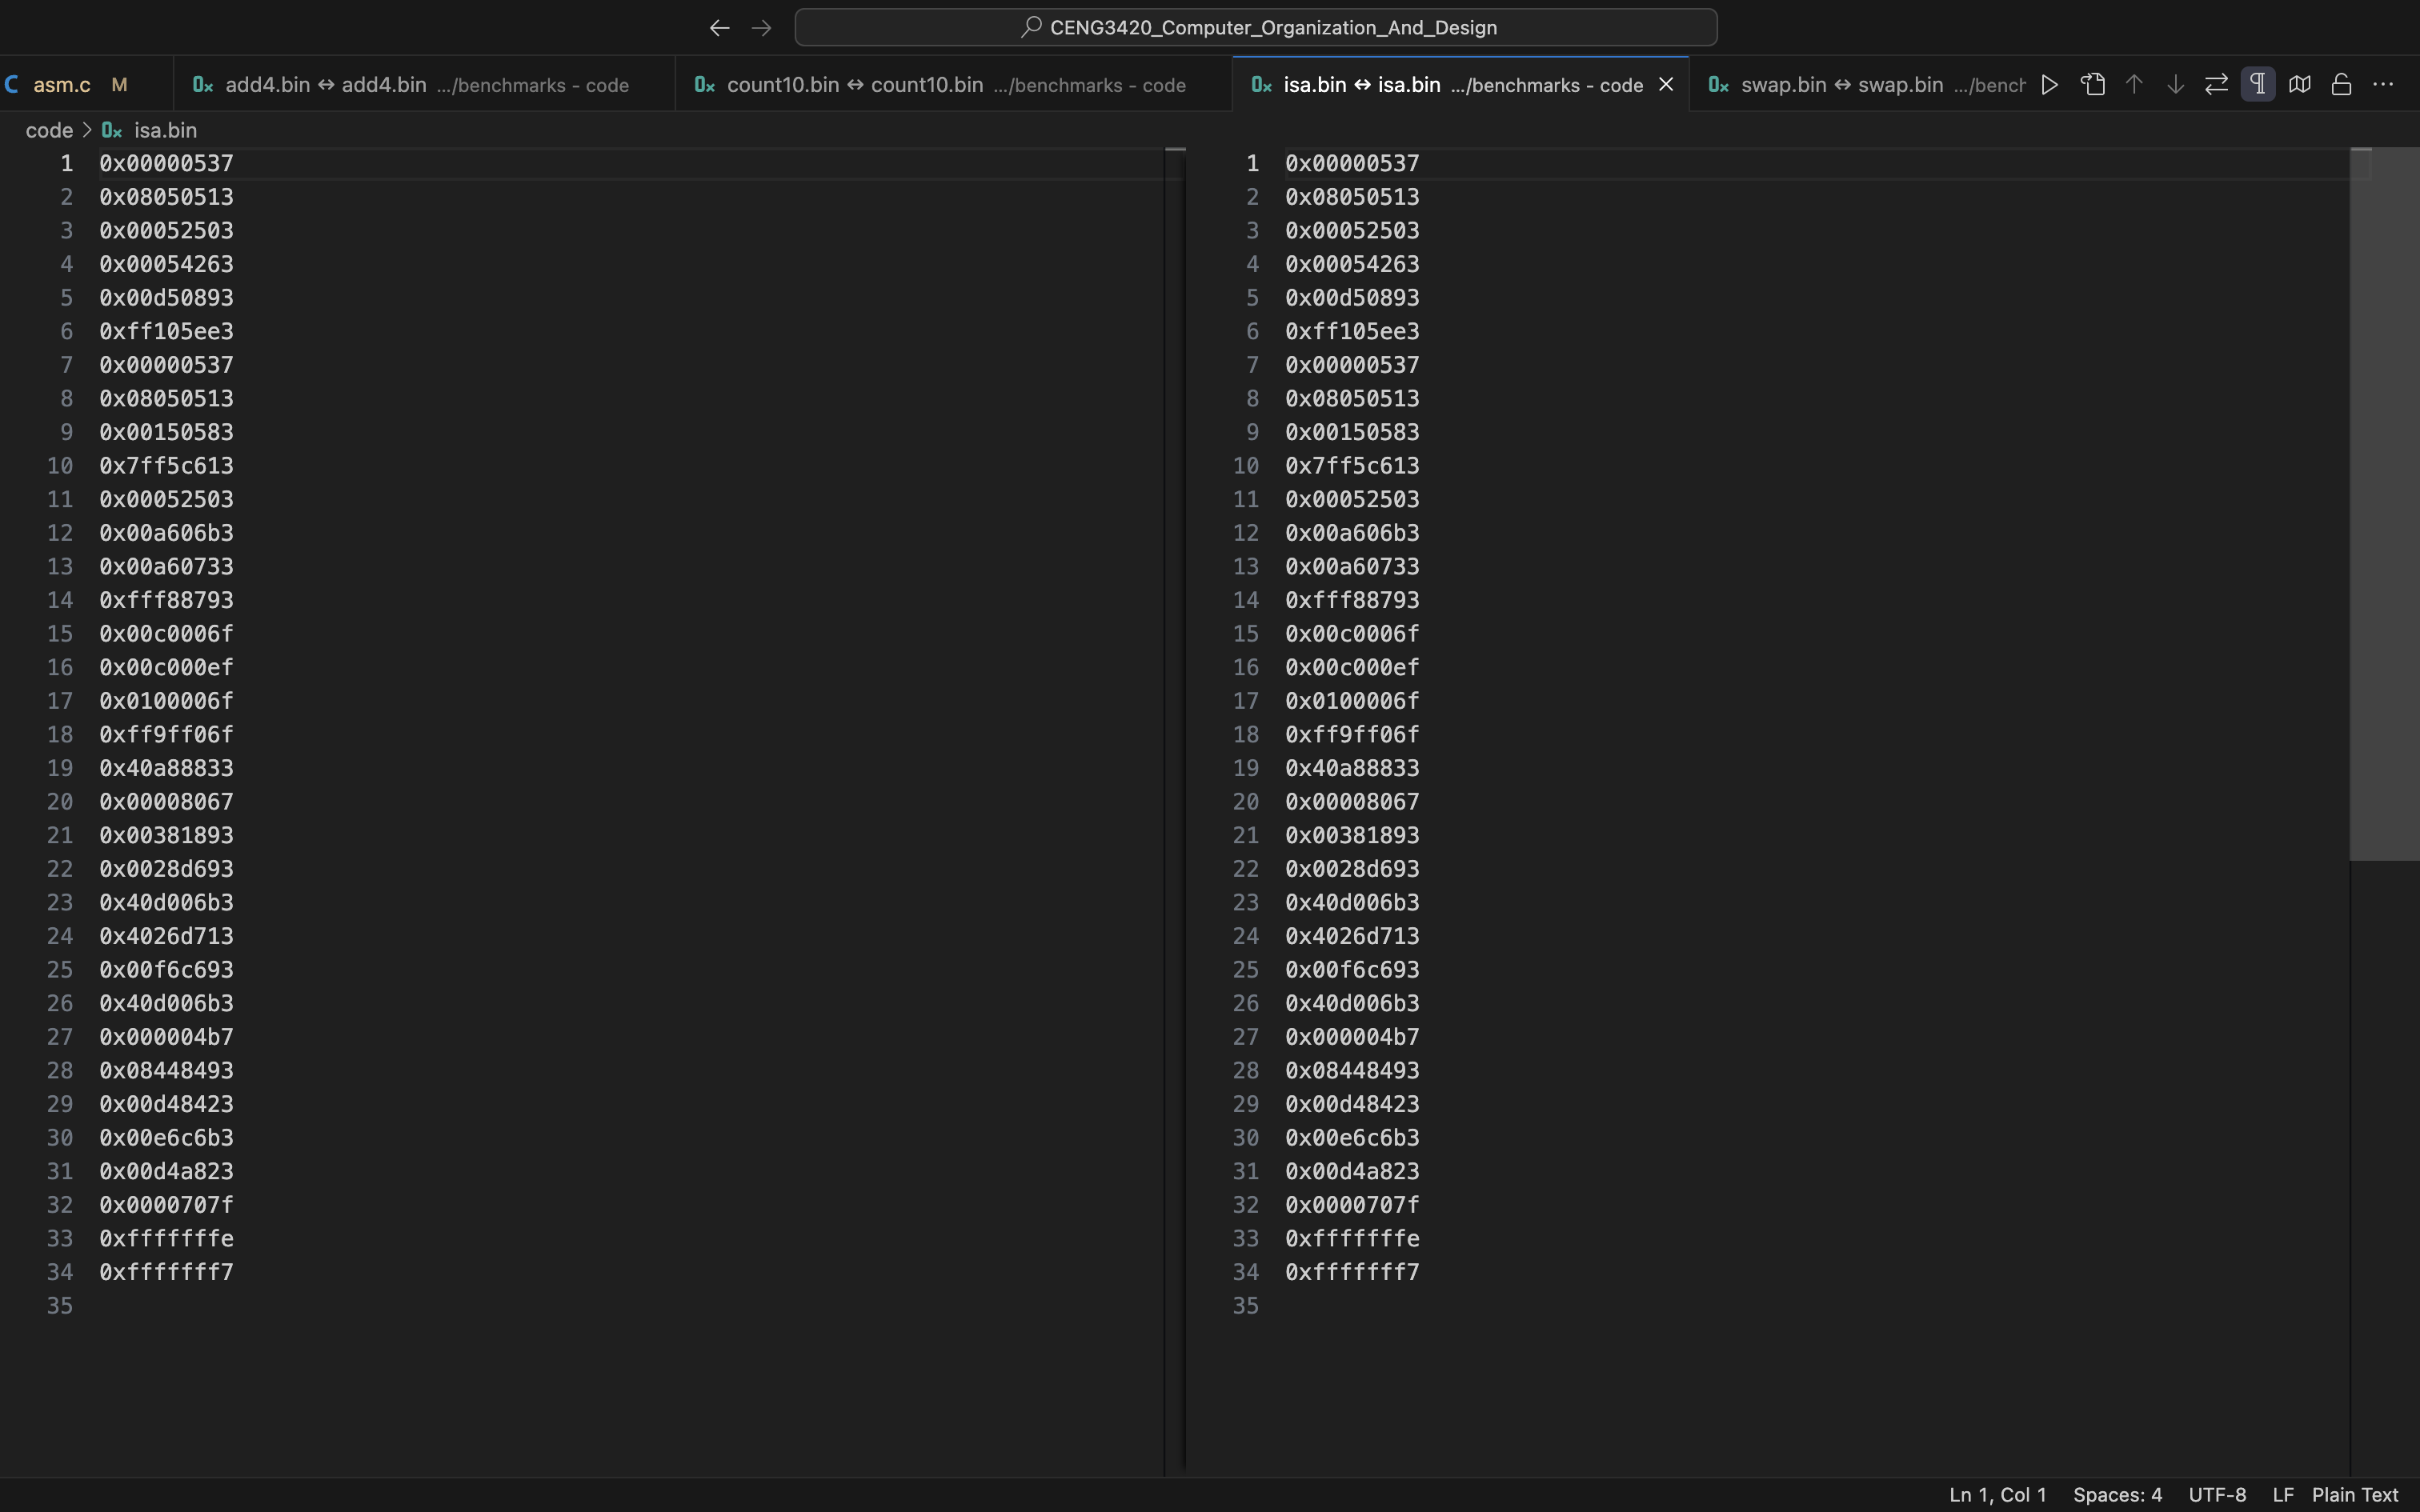
\includegraphics[width=1\linewidth]{../figs/isa.png}
\end{figure}

\begin{figure}[H]
    \caption{swap.bin}
    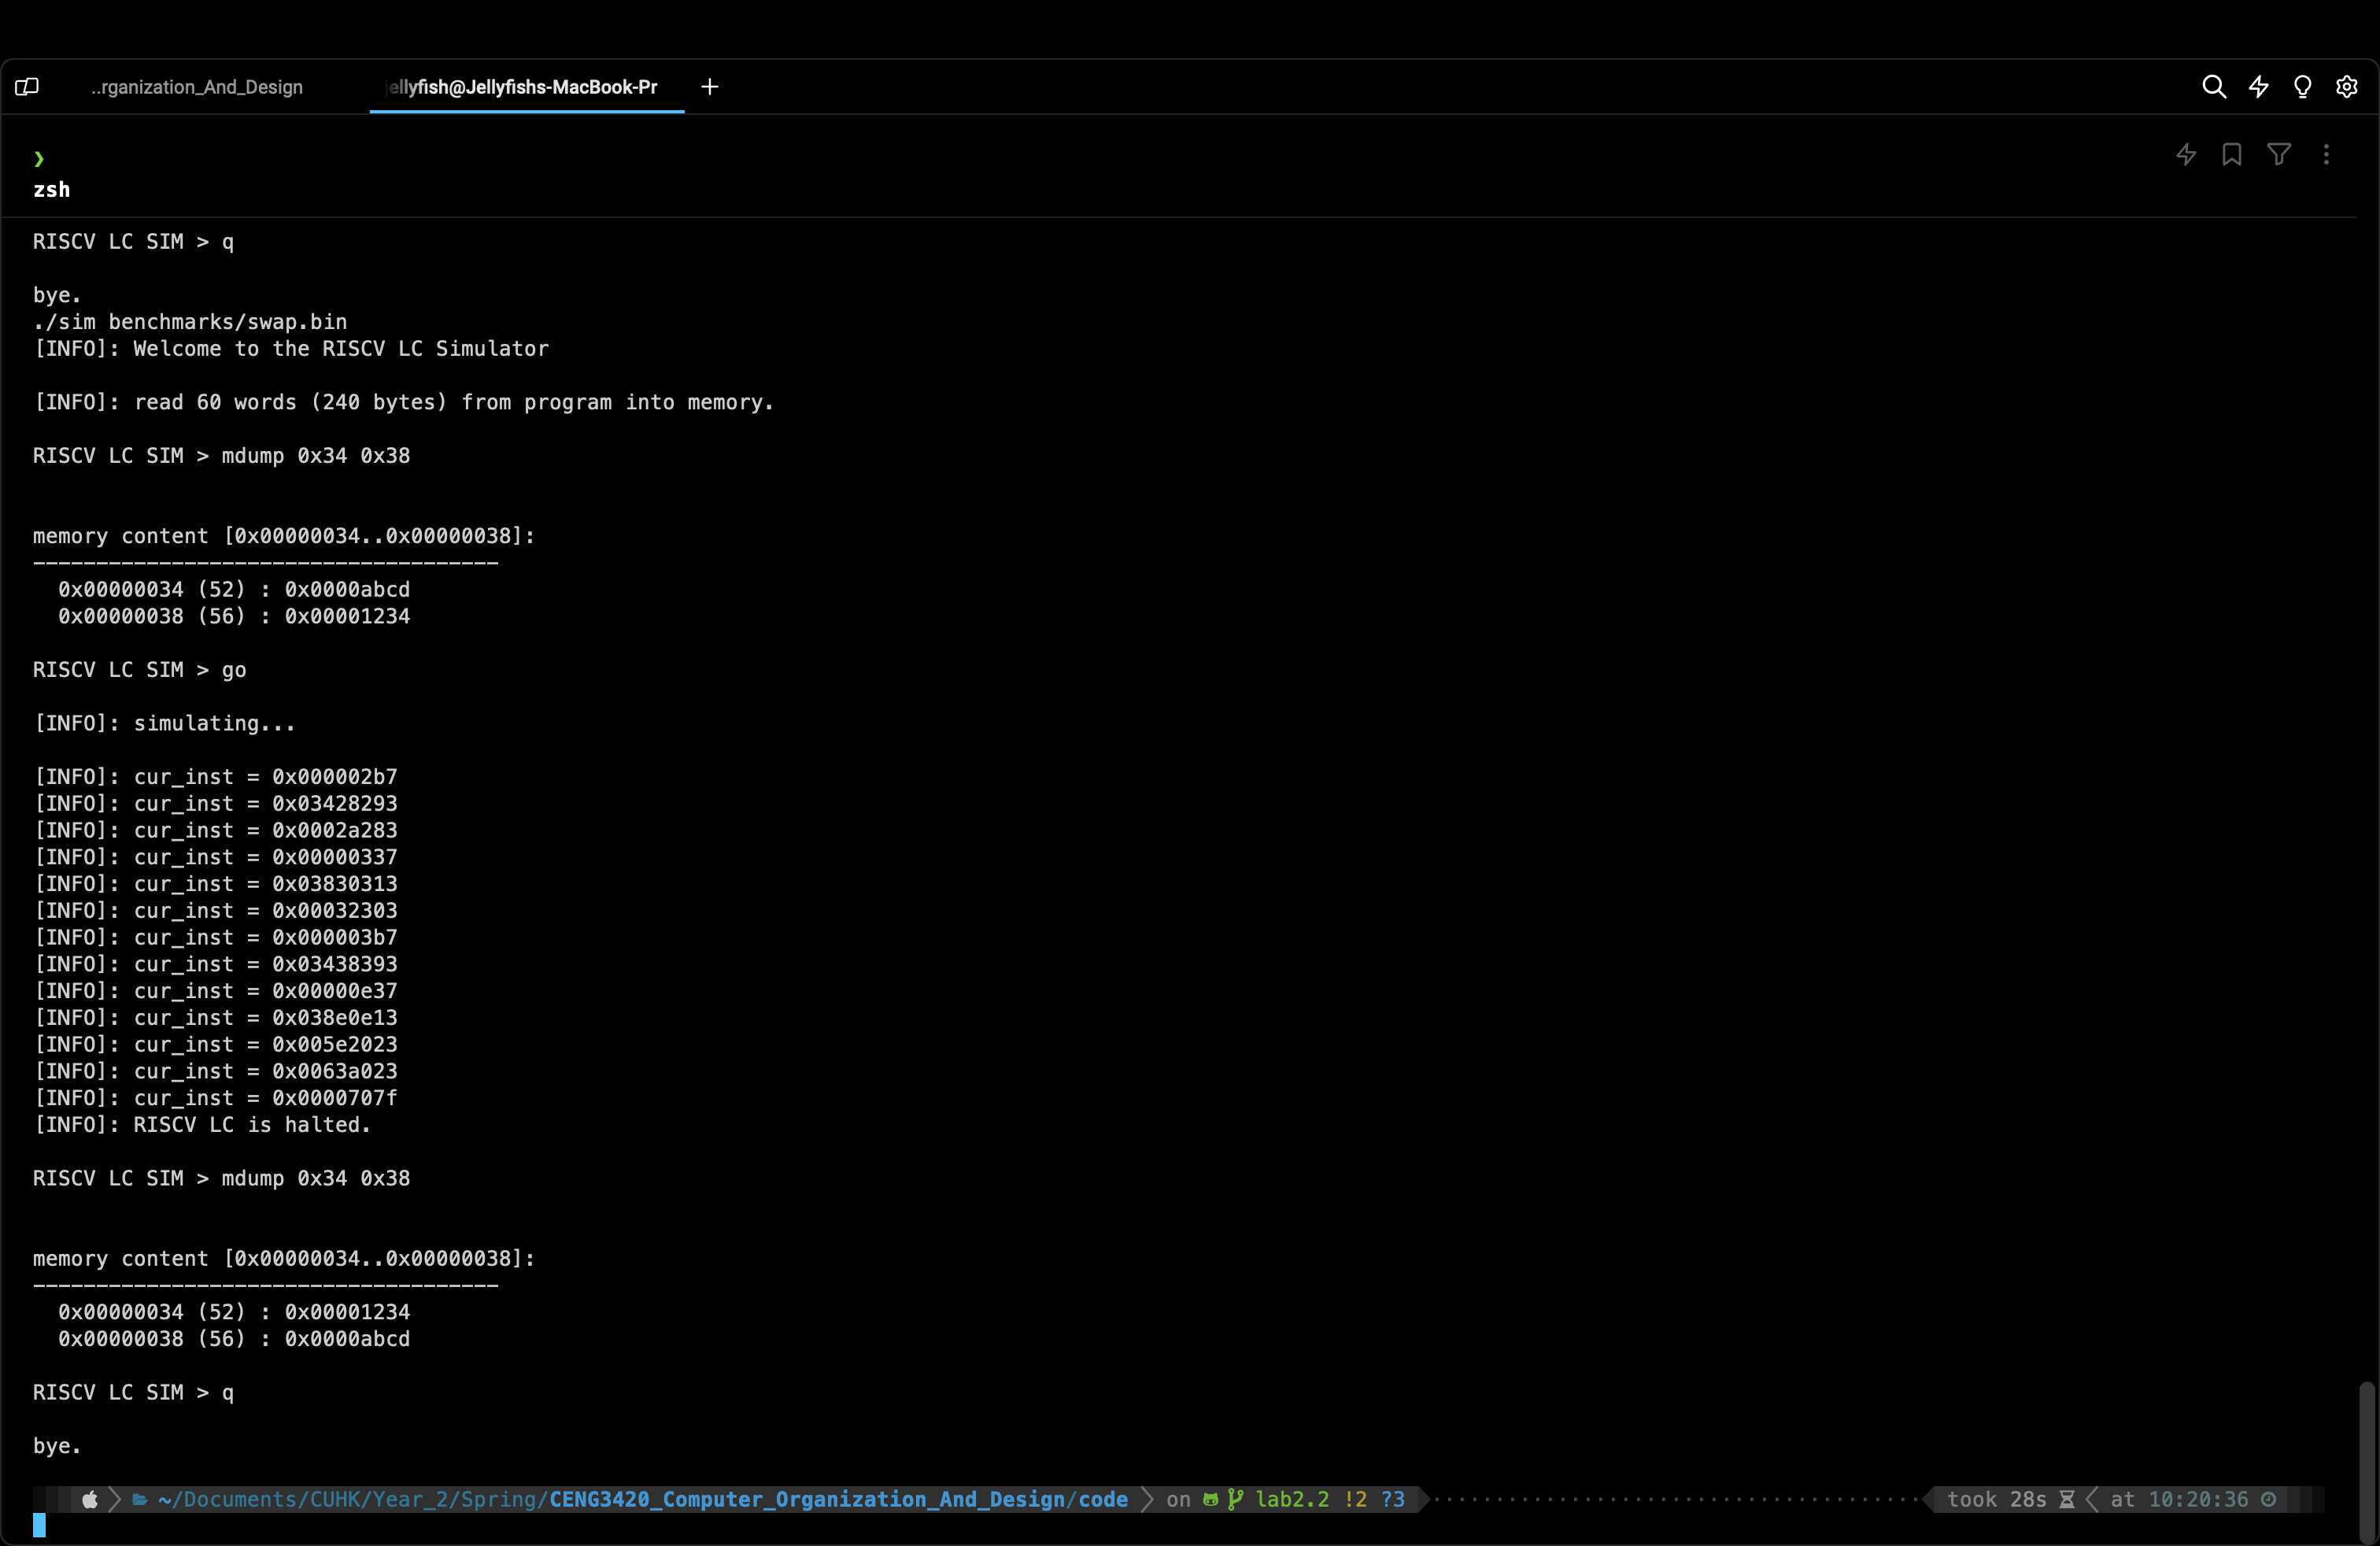
\includegraphics[width=1\linewidth]{../figs/swap.png}
\end{figure}

\end{document}
